\documentclass[twocolumn,10pt]{article}
\title{Slicing 3D solids}
\setlength{\columnsep}{20pt} 
\usepackage{amsmath,hyperref,cancel,graphicx}
 \def\shrinkfactor{0.4}
 \usepackage[margin=1.5cm]{geometry}
\usepackage[usenames,dvipsnames]{color}
 
 \newcommand{\blue}[1]{{\color{Blue}#1}} 
 \newcommand{\purple}[1]{{\color{Purple}#1}} 
 \newcommand{\red}[1]{{\color{Red}#1}} 
 \newcommand{\green}[1]{{\color{Green}#1}} 
 \newcommand{\gray}[1]{{\color{Gray}#1}} 
  \newcommand{\pink}[1]{{\color{Magenta}#1}}   
\RequirePackage[normalem]{ulem} \RequirePackage{color}\definecolor{RED}{rgb}{1,0,0}\definecolor{BLUE}{rgb}{0,0,1} \providecommand{\DIFadd}[1]{{\protect\color{blue}\uwave{#1}}} \providecommand{\DIFdel}[1]{{\protect\color{red}\sout{#1}}}                      \providecommand{\DIFaddbegin}{} \providecommand{\DIFaddend}{} \providecommand{\DIFdelbegin}{} \providecommand{\DIFdelend}{} \providecommand{\DIFaddFL}[1]{\DIFadd{#1}} \providecommand{\DIFdelFL}[1]{\DIFdel{#1}} \providecommand{\DIFaddbeginFL}{} \providecommand{\DIFaddendFL}{} \providecommand{\DIFdelbeginFL}{} \providecommand{\DIFdelendFL}{} 
\begin{document}
\maketitle



\section{\href{https://www.khanacademy.org/devadmin/content/items/x141c0caeea18da08}{x141c0caeea18da08}}

\noindent
The figure below shows a pyramid with a square base. The height of the pyramid is equal to the side of its base. 

**Which \DIFdelbegin \DIFdel{two dimensional shape describes the shape of a vertical slice through the pyramid that does not pass through the center}\DIFdelend \DIFaddbegin \DIFadd{two-dimensional shape will result from the slice shown}\DIFaddend ?**


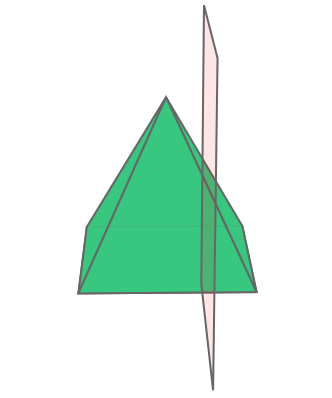
\includegraphics[scale=\shrinkfactor]{figures/5bc3f7ec860f6a648bbe5527e0b891041838f39a.png}

\paragraph{Ans} 

\fbox{ 
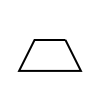
\includegraphics[scale=\shrinkfactor]{figures/462dbf19e63d9954ed7a531f7ea0e2b0379d9bb9.png}

}

 
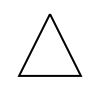
\includegraphics[scale=\shrinkfactor]{figures/d443e0deb4dc18ef30fbf9139d310266f460b66b.png}


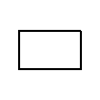
\includegraphics[scale=\shrinkfactor]{figures/0e5042b475e0847d67b74c0482f8e8173f798656.png}


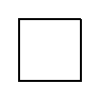
\includegraphics[scale=\shrinkfactor]{figures/4b59a0ece6acc7c19c389e1de534d1df93bf1169.png}



\paragraph{Hint 1}The slice cuts through the pyramid vertically, but not through the center.

\paragraph{Hint 2}The pyramid looks like a triangle when sliced vertically through its center.

When the pyramid is sliced vertically \DIFdelbegin \DIFdel{not passing through the center}\DIFdelend \DIFaddbegin \DIFadd{as shown}\DIFaddend , it looks like a trapezoid.

\paragraph{Hint 3}The shape that we see in an off-centered vertical slice through the pyramid is an isosceles trapezoid.  

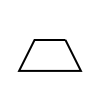
\includegraphics[scale=\shrinkfactor]{figures/462dbf19e63d9954ed7a531f7ea0e2b0379d9bb9.png}




\medskip
\noindent
\textbf{Tags:} {\footnotesize Slicing 3d figures.solid to section, CC.7.G.A.3, SB.7.1.E.4.SR}\\
\textbf{Version:} \DIFdelbegin \DIFdel{10d7ee01.. 2013-10-09
}\DIFdelend \DIFaddbegin \DIFadd{ccaa3213.. 2013-10-16
}\DIFaddend \smallskip\hrule





\section{\href{https://www.khanacademy.org/devadmin/content/items/x4139736ff42aefd2}{x4139736ff42aefd2}}

\noindent
**Which two dimensional shape describes the shape of \DIFdelbegin \DIFdel{a }\DIFdelend \DIFaddbegin \DIFadd{the }\DIFaddend vertical slice through this block of butter \DIFaddbegin \DIFadd{that is shown}\DIFaddend ?**  


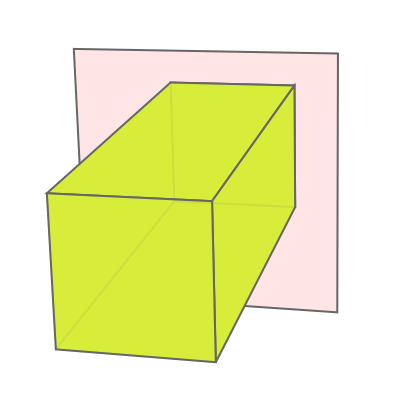
\includegraphics[scale=\shrinkfactor]{figures/750bab6eb7cb314392363d371f78c3ccbc8b4098.png}

\paragraph{Ans} 

\fbox{ 
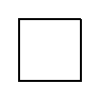
\includegraphics[scale=\shrinkfactor]{figures/4b59a0ece6acc7c19c389e1de534d1df93bf1169.png}

}

 
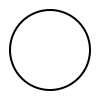
\includegraphics[scale=\shrinkfactor]{figures/9bf34a29bc62816f07057d9e571de844df484cd9.png}


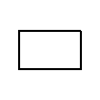
\includegraphics[scale=\shrinkfactor]{figures/0e5042b475e0847d67b74c0482f8e8173f798656.png}


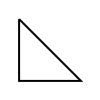
\includegraphics[scale=\shrinkfactor]{figures/02361468f7d85874956214c7a0a119b84a8c2651.png}



\paragraph{Hint 1}The slice cuts through the block of butter vertically \DIFdelbegin \DIFdel{, so the }\DIFdelend \DIFaddbegin \DIFadd{and is parallel to the the front face of the block of butter. The }\DIFaddend shape we'll see in the slice is the same as the front side of the block of butter.

\paragraph{Hint 2}The block of butter has the shape of a right regular prism and its front side is a square.

\paragraph{Hint 3}The shape that we see in \DIFdelbegin \DIFdel{a vertical slice through the butters }\DIFdelend \DIFaddbegin \DIFadd{the vertical slice shown in the figure }\DIFaddend is a square.  

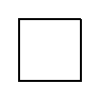
\includegraphics[scale=\shrinkfactor]{figures/4b59a0ece6acc7c19c389e1de534d1df93bf1169.png}



\medskip
\noindent
\textbf{Tags:} {\footnotesize Slicing 3d figures.solid to section, CC.7.G.A.3, SB.7.1.E.4.SR}\\
\textbf{Version:} \DIFdelbegin \DIFdel{4b471f9e.. 2013-10-10
}\DIFdelend \DIFaddbegin \DIFadd{ea607cb9.. 2013-10-16
}\DIFaddend \smallskip\hrule





\section{\href{https://www.khanacademy.org/devadmin/content/items/x72bb801397b54d5e}{x72bb801397b54d5e}}

\noindent
The figure below shows a right rectangular pyramid whose base is a square.

**Which two dimensional shape describes the shape of a horizontal slice through the pyramid?**  


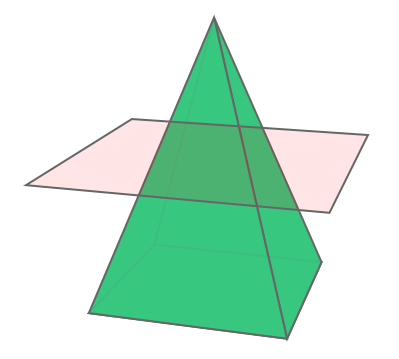
\includegraphics[scale=\shrinkfactor]{figures/3f0ba787b169725c8c4c74a3017b4210d7a511f5.png}

\paragraph{Ans} 

\fbox{ 
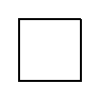
\includegraphics[scale=\shrinkfactor]{figures/4b59a0ece6acc7c19c389e1de534d1df93bf1169.png}

}

 
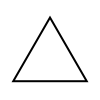
\includegraphics[scale=\shrinkfactor]{figures/15c855a8a232e6c1873c5f46769050a9c13051b8.png}


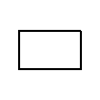
\includegraphics[scale=\shrinkfactor]{figures/0e5042b475e0847d67b74c0482f8e8173f798656.png}


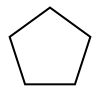
\includegraphics[scale=\shrinkfactor]{figures/498a6b09730fdba2360826c138eeee142e8cccc1.png}



\paragraph{Hint 1}The slice cuts through the pyramid horizontally so the shape we see in the slice is the same as the shape of the base of the pyramid.

\paragraph{Hint 2}Since the shape of the pyramid's base is a square, the shape of the horizontal slice is also a square.

\paragraph{Hint 3}The shape that we see in a horizontal slice through the pyramid is a square.  

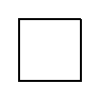
\includegraphics[scale=\shrinkfactor]{figures/4b59a0ece6acc7c19c389e1de534d1df93bf1169.png}



\medskip
\noindent
\textbf{Tags:} {\footnotesize Slicing 3d figures.solid to section, CC.7.G.A.3, SB.7.1.E.4.SR}\\
\textbf{Version:} 0a04d762.. 2013-10-09
\smallskip\hrule





\section{\href{https://www.khanacademy.org/devadmin/content/items/x7b7f9e81dc7e0cea}{x7b7f9e81dc7e0cea}}

\noindent
The figure below shows a right regular prism whose base is a pentagon.

**Which two dimensional shape describes the shape of a horizontal slice through the prism?**  


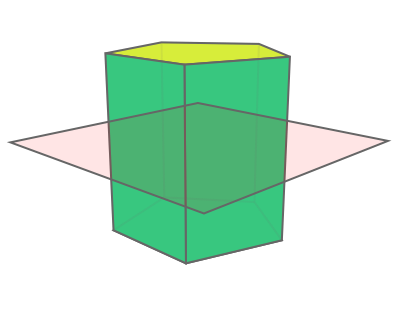
\includegraphics[scale=\shrinkfactor]{figures/fe9352beb31c400cf0f7b64a1efed2b946206cc4.png}

\paragraph{Ans} 

\fbox{ 
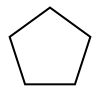
\includegraphics[scale=\shrinkfactor]{figures/498a6b09730fdba2360826c138eeee142e8cccc1.png}

}

 
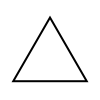
\includegraphics[scale=\shrinkfactor]{figures/15c855a8a232e6c1873c5f46769050a9c13051b8.png}


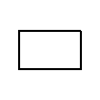
\includegraphics[scale=\shrinkfactor]{figures/0e5042b475e0847d67b74c0482f8e8173f798656.png}


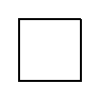
\includegraphics[scale=\shrinkfactor]{figures/4b59a0ece6acc7c19c389e1de534d1df93bf1169.png}



\paragraph{Hint 1}The slice cuts through the prism horizontally so the shape we'll see in the slice is the same as the shape of the base of the prism.

\paragraph{Hint 2}Since the shape of the prism is a pentagon, the shape of the horizontal slice is also a pentagon.

\paragraph{Hint 3}The shape that we'll see in a horizontal slice through the prism is a pentagon.  

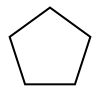
\includegraphics[scale=\shrinkfactor]{figures/498a6b09730fdba2360826c138eeee142e8cccc1.png}



\medskip
\noindent
\textbf{Tags:} {\footnotesize Slicing 3d figures.solid to section, CC.7.G.A.3, SB.7.1.E.4.SR}\\
\textbf{Version:} 9df41222.. 2013-10-09
\smallskip\hrule





\section{\href{https://www.khanacademy.org/devadmin/content/items/x7c120e3f24093a5b}{x7c120e3f24093a5b}}

\noindent
\DIFaddbegin \DIFadd{You're out on a camping trip and you are thinking about the geometry of your tent.
}

\DIFaddend **Which \DIFdelbegin \DIFdel{two dimensional shape describes the shape of a vertical slice through the tent}\DIFdelend \DIFaddbegin \DIFadd{two-dimensional shape will result from the slice shown}\DIFaddend ?**


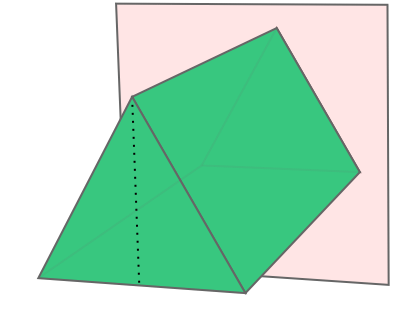
\includegraphics[scale=\shrinkfactor]{figures/416d13238a0976ecc4b9a3a81b3cccd9be6a0c82.png}

\paragraph{Ans} 

\fbox{ 
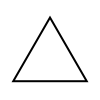
\includegraphics[scale=\shrinkfactor]{figures/15c855a8a232e6c1873c5f46769050a9c13051b8.png}

}

 
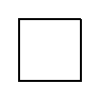
\includegraphics[scale=\shrinkfactor]{figures/4b59a0ece6acc7c19c389e1de534d1df93bf1169.png}


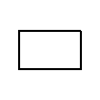
\includegraphics[scale=\shrinkfactor]{figures/0e5042b475e0847d67b74c0482f8e8173f798656.png}


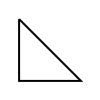
\includegraphics[scale=\shrinkfactor]{figures/02361468f7d85874956214c7a0a119b84a8c2651.png}



\paragraph{Hint 1}The slice cuts through the tent vertically \DIFdelbegin \DIFdel{, so the shape we'll see in the slice is the same as the shape of the  }\DIFdelend \DIFaddbegin \DIFadd{and the direction of the cut is parallel to the }\DIFaddend front of the tent.

\paragraph{Hint 2}The front of the tent (where the zipper is) has the shape of an equilateral triangle.

\paragraph{Hint 3}The shape that we see in a vertical slice through the tent is an equilateral triangle.   

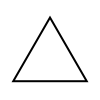
\includegraphics[scale=\shrinkfactor]{figures/15c855a8a232e6c1873c5f46769050a9c13051b8.png}



\medskip
\noindent
\textbf{Tags:} {\footnotesize Slicing 3d figures.solid to section, CC.7.G.A.3, SB.7.1.E.4.SR}\\
\textbf{Version:} \DIFdelbegin \DIFdel{49bacd7b.. 2013-10-10
}\DIFdelend \DIFaddbegin \DIFadd{55c4aad7.. 2013-10-16
}\DIFaddend \smallskip\hrule





\section{\href{https://www.khanacademy.org/devadmin/content/items/x80dc1341b9007790}{x80dc1341b9007790}}

\noindent
The figure below shows a right rectangular prism whose base is a $2 \times 2$ square and whose height is $4$. 

**Which two dimensional shape describes the shape of a horizontal slice through the prism?**  


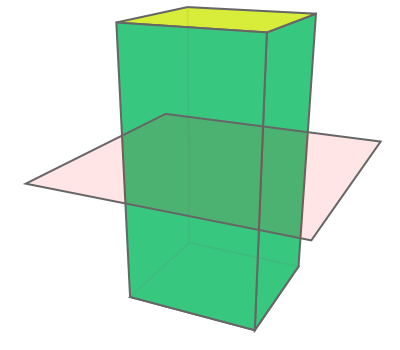
\includegraphics[scale=\shrinkfactor]{figures/ae14dbdd587e39687ed7993df17e46170085a644.png}

\paragraph{Ans} 

\fbox{ 
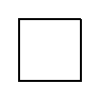
\includegraphics[scale=\shrinkfactor]{figures/4b59a0ece6acc7c19c389e1de534d1df93bf1169.png}

}

 
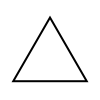
\includegraphics[scale=\shrinkfactor]{figures/15c855a8a232e6c1873c5f46769050a9c13051b8.png}


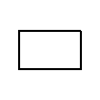
\includegraphics[scale=\shrinkfactor]{figures/0e5042b475e0847d67b74c0482f8e8173f798656.png}


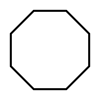
\includegraphics[scale=\shrinkfactor]{figures/7d98a99c75a84da8f748444ad7a3a8053be16a27.png}



\paragraph{Hint 1}The slice cuts through the prism horizontally, so the shape we'll see in the slice is the same as the shape of the base of the prism.

\paragraph{Hint 2}Since the shape of the prism is a $2 \times 2$ square, the shape of the horizontal slice is also a $2 \times 2$ square.

\paragraph{Hint 3}The shape that we see in a horizontal slice through the prism is a square.  

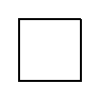
\includegraphics[scale=\shrinkfactor]{figures/4b59a0ece6acc7c19c389e1de534d1df93bf1169.png}



\medskip
\noindent
\textbf{Tags:} {\footnotesize Slicing 3d figures.solid to section, CC.7.G.A.3, SB.7.1.E.4.SR}\\
\textbf{Version:} 4d15a2c6.. 2013-10-09
\smallskip\hrule





\section{\href{https://www.khanacademy.org/devadmin/content/items/xa33f179a801021da}{xa33f179a801021da}}

\noindent
The figure below shows a right rectangular prism whose base is a $2 \times 2$ square and whose height is $4$. 

**Which two dimensional shape describes a vertical slice through the prism?**  


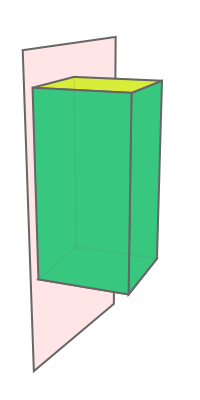
\includegraphics[scale=\shrinkfactor]{figures/75387eceae9780c601f242416bc9fa79e993b9b0.png}

\paragraph{Ans} 

\fbox{ 
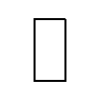
\includegraphics[scale=\shrinkfactor]{figures/225bc3d058cebe2059fc56f78ef80b5f3e0f2da7.png}

}

 
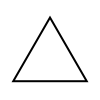
\includegraphics[scale=\shrinkfactor]{figures/15c855a8a232e6c1873c5f46769050a9c13051b8.png}


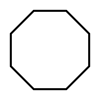
\includegraphics[scale=\shrinkfactor]{figures/7d98a99c75a84da8f748444ad7a3a8053be16a27.png}


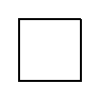
\includegraphics[scale=\shrinkfactor]{figures/4b59a0ece6acc7c19c389e1de534d1df93bf1169.png}



\paragraph{Hint 1}The slice cuts through the prism vertically so the shape we see in the slice is the same as the shape of the side of the prism.

\paragraph{Hint 2}Since the side of the prism is a $2 \times 4$ rectangle, the shape of the vertical slice is also a $2 \times 4$ rectangle.

\paragraph{Hint 3}The shape that we see in a vertical slice through the prism is a rectangle.   

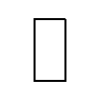
\includegraphics[scale=\shrinkfactor]{figures/225bc3d058cebe2059fc56f78ef80b5f3e0f2da7.png}



\medskip
\noindent
\textbf{Tags:} {\footnotesize Slicing 3d figures.solid to section, CC.7.G.A.3, SB.7.1.E.4.SR}\\
\textbf{Version:} 2ad5b419.. 2013-10-09
\smallskip\hrule





\section{\href{https://www.khanacademy.org/devadmin/content/items/xaaf221c1e7ea291e}{xaaf221c1e7ea291e}}

\noindent
The figure below shows an upside-down pyramid with a square base.

**Which two dimensional shape describes the shape of a horizontal slice through the pyramid?**  


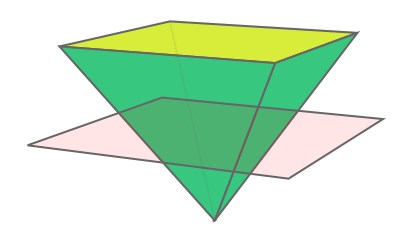
\includegraphics[scale=\shrinkfactor]{figures/76b893a13f023803c8c76f7ab435acb2361604b4.png}

\paragraph{Ans} 

\fbox{ 
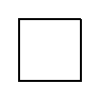
\includegraphics[scale=\shrinkfactor]{figures/4b59a0ece6acc7c19c389e1de534d1df93bf1169.png}

}

 
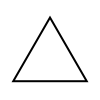
\includegraphics[scale=\shrinkfactor]{figures/15c855a8a232e6c1873c5f46769050a9c13051b8.png}


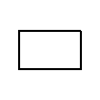
\includegraphics[scale=\shrinkfactor]{figures/0e5042b475e0847d67b74c0482f8e8173f798656.png}


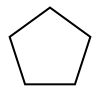
\includegraphics[scale=\shrinkfactor]{figures/498a6b09730fdba2360826c138eeee142e8cccc1.png}



\paragraph{Hint 1}The slice cuts through the pyramid horizontally so the shape we see in the slice is the same as the shape of the base of the pyramid.

\paragraph{Hint 2}Since the shape of the pyramid's base is a square, the shape of the horizontal slice is also a square.

\paragraph{Hint 3}The shape that we see in a horizontal slice through the upside-down pyramid is a square.  

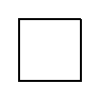
\includegraphics[scale=\shrinkfactor]{figures/4b59a0ece6acc7c19c389e1de534d1df93bf1169.png}



\medskip
\noindent
\textbf{Tags:} {\footnotesize Slicing 3d figures.solid to section, CC.7.G.A.3, SB.7.1.E.4.SR}\\
\textbf{Version:} ba6e79ec.. 2013-10-10
\smallskip\hrule





\section{\href{https://www.khanacademy.org/devadmin/content/items/xc8ec7679f407c09d}{xc8ec7679f407c09d}}

\noindent
The figure below shows a prism whose base is an equilateral triangle.

**Which two dimensional shape describes the shape of a horizontal slice through the prism?**  


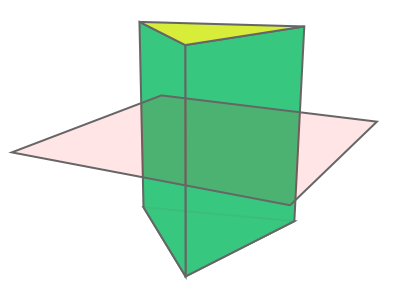
\includegraphics[scale=\shrinkfactor]{figures/f12c7d1a9a889fab96bfd40a772ef7d4478018ad.png}

\paragraph{Ans} 

\fbox{ 
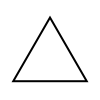
\includegraphics[scale=\shrinkfactor]{figures/15c855a8a232e6c1873c5f46769050a9c13051b8.png}

}

 
\includegraphics[scale=\shrinkfactor]{figures/4b59a0ece6acc7c19c389e1de534d1df93bf1169.png}


\includegraphics[scale=\shrinkfactor]{figures/0e5042b475e0847d67b74c0482f8e8173f798656.png}


\includegraphics[scale=\shrinkfactor]{figures/7d98a99c75a84da8f748444ad7a3a8053be16a27.png}



\paragraph{Hint 1}The slice cuts through the prism horizontally, so the shape we'll see in the slice is the same as the shape of the base of the prism.

\paragraph{Hint 2}Since the base of the prism is an equilateral triangle, the shape of the horizontal slice is also an equilateral triangle.

\paragraph{Hint 3}The shape that we see in a horizontal slice through the prism is an equilateral triangle.   

\includegraphics[scale=\shrinkfactor]{figures/15c855a8a232e6c1873c5f46769050a9c13051b8.png}



\medskip
\noindent
\textbf{Tags:} {\footnotesize Slicing 3d figures.solid to section, CC.7.G.A.3, SB.7.1.E.4.SR}\\
\textbf{Version:} 38a72235.. 2013-10-09
\smallskip\hrule





\section{\href{https://www.khanacademy.org/devadmin/content/items/xddab61063efd799b}{xddab61063efd799b}}

\noindent
The figure below shows a pyramid with a square base. The height of the pyramid is equal to the side of its base. 

**Which two dimensional shape describes the shape of a vertical slice through the center of the  pyramid?**  


\includegraphics[scale=\shrinkfactor]{figures/5886f271642379937f772874924e3bcee68b664a.png}

\paragraph{Ans} 

\fbox{ 
\includegraphics[scale=\shrinkfactor]{figures/d443e0deb4dc18ef30fbf9139d310266f460b66b.png}

}

 

\includegraphics[scale=\shrinkfactor]{figures/4b59a0ece6acc7c19c389e1de534d1df93bf1169.png}


\includegraphics[scale=\shrinkfactor]{figures/0e5042b475e0847d67b74c0482f8e8173f798656.png}


\includegraphics[scale=\shrinkfactor]{figures/0245164f3f4897772e76d361f955075a80732b03.png}



\paragraph{Hint 1}The slice cuts through the pyramid vertically and passes through the center of the pyramid.

What is the shape of the pyramid when you look at it from the side?

\paragraph{Hint 2}The pyramid looks like a triangle when sliced vertically through its center.

\paragraph{Hint 3}The shape that we'll see in a vertical slice through the center of the pyramid is an isosceles triangle whose height is equal to the length of its base.  

\includegraphics[scale=\shrinkfactor]{figures/d443e0deb4dc18ef30fbf9139d310266f460b66b.png}




\medskip
\noindent
\textbf{Tags:} {\footnotesize Slicing 3d figures.solid to section, CC.7.G.A.3, SB.7.1.E.4.SR}\\
\textbf{Version:} 0c35e7de.. 2013-10-09
\smallskip\hrule





\section{\href{https://www.khanacademy.org/devadmin/content/items/x209d34a33212eb67}{x209d34a33212eb67}}

\noindent
Taking a horizontal slice through a three dimensional solid produces a two dimensional shape.

**When sliced horizontally, which of the following solids would produce this two dimensional shape?**   

\includegraphics[scale=\shrinkfactor]{figures/788a8b56b0b7607b1ee5b54e7626cf4b802e373f.png} 


\paragraph{Ans} 

\fbox{ 
\includegraphics[scale=\shrinkfactor]{figures/df7e52cb3a541015199076ff457ee6bdda3a663c.png}

}

 
\includegraphics[scale=\shrinkfactor]{figures/5f94871e71f674049268d58ac56b3de4dfa3a3ba.png}


\includegraphics[scale=\shrinkfactor]{figures/714aa411c23dfb02df032183d703d78050ecb5ae.png}


\includegraphics[scale=\shrinkfactor]{figures/8e0bce39d089e690c82fd2275ed9e00339fd8202.png}



\paragraph{Hint 1}The shape we see in the two dimensional slice is a triangle. Therefore, the solid which was sliced must have a triangular base. 

\paragraph{Hint 2}Which of the solids in the choices has a triangular base?

\paragraph{Hint 3}Only the right prism with a triangular base would produce a triangle when sliced horizontally.


\includegraphics[scale=\shrinkfactor]{figures/df7e52cb3a541015199076ff457ee6bdda3a663c.png}



\medskip
\noindent
\textbf{Tags:} {\footnotesize Slicing 3d figures.section to solid, CC.7.G.A.3, SB.7.1.E.4.SR}\\
\textbf{Version:} 4f799bdd.. 2013-10-09
\smallskip\hrule





\section{\href{https://www.khanacademy.org/devadmin/content/items/x2e7aee12e3895c4c}{x2e7aee12e3895c4c}}

\noindent
A vertical slice through a three dimensional solid produces a two dimensional shape.

**When sliced vertically, which of the following solids would produce this two dimensional shape?**   

\includegraphics[scale=\shrinkfactor]{figures/9a01e5fee86b7569b86f7e8f116595d328925a8c.png} 


\paragraph{Ans} 

\fbox{ 
\includegraphics[scale=\shrinkfactor]{figures/49b99cca0c4e580ceaef3d4fd5842ea463191ce8.png}

}

 
\includegraphics[scale=\shrinkfactor]{figures/5f94871e71f674049268d58ac56b3de4dfa3a3ba.png}


\includegraphics[scale=\shrinkfactor]{figures/714aa411c23dfb02df032183d703d78050ecb5ae.png}


\includegraphics[scale=\shrinkfactor]{figures/df7e52cb3a541015199076ff457ee6bdda3a663c.png}



\paragraph{Hint 1}The shape we see in the two dimensional slice is an isosceles trapezoid. It is a trapezoid because it has two parallel sides and it is isosceles because its left side looks like the mirror image of the right side, like an isosceles triangle.

\paragraph{Hint 2}Which of the solids in the choices would produce a shape with sloping sides when sliced vertically?

\paragraph{Hint 3}The triangular, square, and pentagonal prisms all have vertical sides so slicing them vertically cannot produce a shape with sloping sides.

\paragraph{Hint 4}Only a vertical slice through the pyramid produces a two dimensional shape with sloping sides.


\includegraphics[scale=\shrinkfactor]{figures/49b99cca0c4e580ceaef3d4fd5842ea463191ce8.png}

To produce an isosceles trapezoid, we can slice the pyramid making a cut that does not pass through the center.


\includegraphics[scale=\shrinkfactor]{figures/5c4f5d18cffbd9888619838aea65c59f3f17f1d0.png}



\medskip
\noindent
\textbf{Tags:} {\footnotesize Slicing 3d figures.section to solid, CC.7.G.A.3, SB.7.1.E.4.SR}\\
\textbf{Version:} 91e6a838.. 2013-10-09
\smallskip\hrule





\section{\href{https://www.khanacademy.org/devadmin/content/items/x2ea82a3291511b2e}{x2ea82a3291511b2e}}

\noindent
A vertical slice through a three dimensional solid produces a two dimensional shape.

**When sliced vertically, which of the following solids would produce this two dimensional shape?**   

\includegraphics[scale=\shrinkfactor]{figures/7ccd247b0c79be3865322f7b79cbc84002ad5412.png} 


\paragraph{Ans} 

\fbox{ 
\includegraphics[scale=\shrinkfactor]{figures/2ebec88f0b30eab2455be53549a16e7fc9469bd3.png}

}

 
\includegraphics[scale=\shrinkfactor]{figures/49b99cca0c4e580ceaef3d4fd5842ea463191ce8.png}


\DIFdelbegin \DIFdelend \DIFaddbegin \includegraphics[scale=\shrinkfactor]{figures/a31c76eab3504d9cc594b491934c4893556f58c4.png}
\DIFaddend 


\includegraphics[scale=\shrinkfactor]{figures/47526769b6e12df6ce07410a61d504c7f1d84475.png}



\paragraph{Hint 1}The shape we see in the two dimensional slice is a rectangle.

\paragraph{Hint 2}Which of the solids in the choices would produce a rectangular shape when sliced vertically? 

A vertical slice through the pyramids would produce a shape with sloping sides, not a rectangle.

\DIFdelbegin \DIFdel{A vertical slice through a cube produces a square, not a rectangle.
}
\DIFdelend \paragraph{Hint 3}Only the prism \DIFdelbegin \DIFdel{with a square base }\DIFdelend could produces the rectangular shape when sliced vertically.


\includegraphics[scale=\shrinkfactor]{figures/2ebec88f0b30eab2455be53549a16e7fc9469bd3.png}



\medskip
\noindent
\textbf{Tags:} {\footnotesize Slicing 3d figures.section to solid, CC.7.G.A.3, SB.7.1.E.4.SR}\\
\textbf{Version:} \DIFdelbegin \DIFdel{9c86b143.. 2013-10-09
}\DIFdelend \DIFaddbegin \DIFadd{34d5b5f3.. 2013-10-16
}\DIFaddend \smallskip\hrule





\section{\href{https://www.khanacademy.org/devadmin/content/items/x4f1f8eb1e5cd00ec}{x4f1f8eb1e5cd00ec}}

\noindent
A horizontal slice through a three dimensional solid produces a two dimensional shape.

**When sliced horizontally, which of the following solids would produce this two dimensional shape?**   

\includegraphics[scale=\shrinkfactor]{figures/c3a4fe85ac002ccb07495385394da51d1dcff923.png} 


\paragraph{Ans} 


\includegraphics[scale=\shrinkfactor]{figures/df7e52cb3a541015199076ff457ee6bdda3a663c.png}


\includegraphics[scale=\shrinkfactor]{figures/5f94871e71f674049268d58ac56b3de4dfa3a3ba.png}


\includegraphics[scale=\shrinkfactor]{figures/714aa411c23dfb02df032183d703d78050ecb5ae.png}

\fbox{ 
\includegraphics[scale=\shrinkfactor]{figures/994232bee673b9d41efe1aa168ac2544d5531e55.png}

}

 

\paragraph{Hint 1}The shape we see in the two dimensional slice is hexagon.

\paragraph{Hint 2}Which of the solids in the choices would produce a hexagonal shape when sliced horizontally? 

Which of the solids has a hexagonal base?

\paragraph{Hint 3}The prism with a hexagonal base would produces a hexagon when sliced horizontally.


\includegraphics[scale=\shrinkfactor]{figures/994232bee673b9d41efe1aa168ac2544d5531e55.png}



\medskip
\noindent
\textbf{Tags:} {\footnotesize Slicing 3d figures.section to solid, CC.7.G.A.3, SB.7.1.E.4.SR}\\
\textbf{Version:} da238784.. 2013-10-09
\smallskip\hrule





\section{\href{https://www.khanacademy.org/devadmin/content/items/x728cd6c47f90fd12}{x728cd6c47f90fd12}}

\noindent
A vertical slice through a three dimensional solid produces a two dimensional shape.

**When sliced vertically, which of the following solids would produce this two dimensional shape?**   

\includegraphics[scale=\shrinkfactor]{figures/820f1a9b52329001eaf7845a5d6661adb18f27b8.png} 


\paragraph{Ans} 

\fbox{ 
\includegraphics[scale=\shrinkfactor]{figures/14c5d54ad8e900843fbf2ef335f5a5a14d651f5b.png}

}

 
\includegraphics[scale=\shrinkfactor]{figures/2ebec88f0b30eab2455be53549a16e7fc9469bd3.png}


\includegraphics[scale=\shrinkfactor]{figures/8c9b8f93c15337437fb9789bed7ef67cdfe13e01.png}


\includegraphics[scale=\shrinkfactor]{figures/df7e52cb3a541015199076ff457ee6bdda3a663c.png}



\paragraph{Hint 1}The shape we see in the two dimensional slice is an equilateral triangle.

\paragraph{Hint 2}Which of the solids in the choices would produce a triangular shape when sliced vertically? 

Slicing the right rectangular prism and the cube \DIFaddbegin \DIFadd{vertically }\DIFaddend will produce rectangular shapes\DIFdelbegin \DIFdel{so there are the correct answer}\DIFdelend \DIFaddbegin \DIFadd{, not triangles}\DIFaddend .

A **horizontal** slice through the upright triangular prism will produce a triangular shape, but the question states that we took a vertical slice.
A vertical slice through the upright triangular prism looks like a rectangle, so it is not the correct answer either.

\paragraph{Hint 3}The horizontal triangular prism will produce an equilateral triangle when sliced vertically.  

\includegraphics[scale=\shrinkfactor]{figures/14c5d54ad8e900843fbf2ef335f5a5a14d651f5b.png}



\medskip
\noindent
\textbf{Tags:} {\footnotesize Slicing 3d figures.section to solid, CC.7.G.A.3, SB.7.1.E.4.SR}\\
\textbf{Version:} \DIFdelbegin \DIFdel{e18dd330.. 2013-10-10
}\DIFdelend \DIFaddbegin \DIFadd{01f67a53.. 2013-10-13
}\DIFaddend \smallskip\hrule





\section{\href{https://www.khanacademy.org/devadmin/content/items/x8bf3dcc1812f07b6}{x8bf3dcc1812f07b6}}

\noindent
A horizontal slice through a three dimensional solid produces a two dimensional shape.

**When sliced horizontally, which of the following solids would produce this two dimensional shape?**   

\includegraphics[scale=\shrinkfactor]{figures/f6f3d7d862af181c9db9337ad959b4868e25835c.png} 


\paragraph{Ans} 


\includegraphics[scale=\shrinkfactor]{figures/df7e52cb3a541015199076ff457ee6bdda3a663c.png}


\includegraphics[scale=\shrinkfactor]{figures/5f94871e71f674049268d58ac56b3de4dfa3a3ba.png}

\fbox{ 
\includegraphics[scale=\shrinkfactor]{figures/714aa411c23dfb02df032183d703d78050ecb5ae.png}

}

 
\includegraphics[scale=\shrinkfactor]{figures/994232bee673b9d41efe1aa168ac2544d5531e55.png}



\paragraph{Hint 1}The shape we see in the two dimensional slice is a pentagon.

\paragraph{Hint 2}Which of the solids in the choices would produce a pentagonal shape when sliced horizontally? 

Which of the solids has a pentagonal base?

\paragraph{Hint 3}The prism with a pentagonal base would produces a pentagonal shape when sliced horizontally.


\includegraphics[scale=\shrinkfactor]{figures/714aa411c23dfb02df032183d703d78050ecb5ae.png}



\medskip
\noindent
\textbf{Tags:} {\footnotesize Slicing 3d figures.section to solid, CC.7.G.A.3, SB.7.1.E.4.SR}\\
\textbf{Version:} 03513d58.. 2013-10-09
\smallskip\hrule





\section{\href{https://www.khanacademy.org/devadmin/content/items/xa63d03bcdc40499a}{xa63d03bcdc40499a}}

\noindent
A horizontal slice through a three dimensional solid produces a two dimensional shape.

**When sliced horizontally, which of the following solids would produce this two dimensional shape?**   

\includegraphics[scale=\shrinkfactor]{figures/cb9770c6111993072743c8d1e6fe4ea316f56162.png} 


\paragraph{Ans} 


\includegraphics[scale=\shrinkfactor]{figures/df7e52cb3a541015199076ff457ee6bdda3a663c.png}

\fbox{ 
\includegraphics[scale=\shrinkfactor]{figures/5f94871e71f674049268d58ac56b3de4dfa3a3ba.png}

}

 
\includegraphics[scale=\shrinkfactor]{figures/714aa411c23dfb02df032183d703d78050ecb5ae.png}


\includegraphics[scale=\shrinkfactor]{figures/994232bee673b9d41efe1aa168ac2544d5531e55.png}



\paragraph{Hint 1}The shape we see in the two dimensional slice is a square.

\paragraph{Hint 2}Which of the solids in the choices would produce a square shape when sliced horizontally? 

Which of the solids has a square base?

\paragraph{Hint 3}The prism with a square base would produces a square shape when sliced horizontally.


\includegraphics[scale=\shrinkfactor]{figures/5f94871e71f674049268d58ac56b3de4dfa3a3ba.png}



\medskip
\noindent
\textbf{Tags:} {\footnotesize Slicing 3d figures.section to solid, CC.7.G.A.3, SB.7.1.E.4.SR}\\
\textbf{Version:} 9287e51c.. 2013-10-09
\smallskip\hrule





\section{\href{https://www.khanacademy.org/devadmin/content/items/xb0b26af2552ebf85}{xb0b26af2552ebf85}}

\noindent
A vertical slice through a three dimensional solid produces a two dimensional shape.

**When sliced vertically, which of the following solids would produce this two dimensional shape?**   

\includegraphics[scale=\shrinkfactor]{figures/151efcfa25040f7476db2bf2a762a1067d899304.png} 

\paragraph{Ans} 

\fbox{ 
\includegraphics[scale=\shrinkfactor]{figures/49b99cca0c4e580ceaef3d4fd5842ea463191ce8.png}

}

 
\includegraphics[scale=\shrinkfactor]{figures/5f94871e71f674049268d58ac56b3de4dfa3a3ba.png}


\includegraphics[scale=\shrinkfactor]{figures/714aa411c23dfb02df032183d703d78050ecb5ae.png}


\includegraphics[scale=\shrinkfactor]{figures/8c9b8f93c15337437fb9789bed7ef67cdfe13e01.png}



\paragraph{Hint 1}The shape we see in the two dimensional slice is a triangle.

\paragraph{Hint 2}Which of the solids in the choices would produce a triangle when sliced vertically?

\paragraph{Hint 3}The three prisms all have vertical sides so slicing them vertically will not produce a triangular shape.

\paragraph{Hint 4}Only a vertical slice through the center of the pyramid produces a triangular shape.


\includegraphics[scale=\shrinkfactor]{figures/49b99cca0c4e580ceaef3d4fd5842ea463191ce8.png}




\medskip
\noindent
\textbf{Tags:} {\footnotesize Slicing 3d figures.section to solid, CC.7.G.A.3, SB.7.1.E.4.SR}\\
\textbf{Version:} b50815e2.. 2013-10-09
\smallskip\hrule





\section{\href{https://www.khanacademy.org/devadmin/content/items/x462b5e87a5ace1db}{x462b5e87a5ace1db}}

\noindent
The figure below shows a pyramid whose base is a $6\times 6$ square and whose height is $6$.   

**Draw \DIFdelbegin \DIFdel{the shape you will see if you take }\DIFdelend \DIFaddbegin \DIFadd{a shape you would see when taking }\DIFaddend a horizontal slice through the pyramid.**


\includegraphics[scale=\shrinkfactor]{figures/4e6db0b061f7d0aaab47e90516b4d1a2b8bb2023.png}

[[? interactive-graph 1]] 

\paragraph{Ans} Move the points to draw the shape. 

\paragraph{Hint 1}The slice cuts through the pyramid horizontally, so the shape we'll see in the slice is the same as the shape of the base of the pyramid.

\paragraph{Hint 2}The base of the pyramid is square, therefore a horizontal slice through the pyramid will also look like a square.

\paragraph{Hint 3}Depending on the height where we make the cut, the square in the slice will have different size. A slice near the top of the pyramid will look like a very small square, whereas a slice near the base of the pyramid will be larger**.**

A horizontal slice through the middle of the pyramid (at halfway of its height) will look like a $3 \times 3$ square:    

\includegraphics[scale=\shrinkfactor]{figures/339319c697846538f4f62770f5fc3cc189f26e88.png}



\medskip
\noindent
\textbf{Tags:} {\footnotesize Slicing 3d figures.draw section, CC.7.G.A.3, SB.7.1.E.4.SR}\\
\textbf{Version:} \DIFdelbegin \DIFdel{2d312080.. 2013-10-09
}\DIFdelend \DIFaddbegin \DIFadd{c724949e.. 2013-10-16
}\DIFaddend \smallskip\hrule





\section{\href{https://www.khanacademy.org/devadmin/content/items/x581101157bf5ca32}{x581101157bf5ca32}}

\noindent
The figure below shows a cube with side length $3$.   

**Draw the shape you will see if you take a horizontal slice through the cube.**


\includegraphics[scale=\shrinkfactor]{figures/f0b7654c0b53908504fb120f51f2b50f3f8fd955.png}

[[? interactive-graph 1]]


\paragraph{Ans} Move the points to draw the shape. 

\paragraph{Hint 1}The slice cuts through the cube horizontally, so the shape we'll see in the slice is the same as the shape of the base of the cube.

\paragraph{Hint 2}Since the cube case side length $3$, the base of the cube has the shape of a $3 \times 3$ square. 


\paragraph{Hint 3}The shape of the horizontal slice through the cube is a $3 \times 3$ square:  

\includegraphics[scale=\shrinkfactor]{figures/225c50ae63dfe1e1e5efd66c940ebfbbd9e44ca2.png}



\medskip
\noindent
\textbf{Tags:} {\footnotesize Slicing 3d figures.draw section, CC.7.G.A.3, SB.7.1.E.4.SR}\\
\textbf{Version:} a83fecd0.. 2013-10-09
\smallskip\hrule





\section{\href{https://www.khanacademy.org/devadmin/content/items/x6b70eb108befb974}{x6b70eb108befb974}}

\noindent
The figure below shows prism whose base is a $3\times 3$ square and whose height is $6$.   

**Draw the shape you will see if you take a vertical slice through the prism.**   
\DIFaddbegin \DIFadd{Assume the vertical slice is parallel to one of the sides of the prism.
}\DIFaddend 


\includegraphics[scale=\shrinkfactor]{figures/94bf14f4775048a20e633abd42558d8e108ecfab.png}

[[? interactive-graph 1]] 

\paragraph{Ans} Move the points to draw the shape. 

\paragraph{Hint 1}The slice cuts through the prism vertically \DIFaddbegin \DIFadd{parallel to one of the sides}\DIFaddend , so the shape we'll see in the slice is the same as the shape of the side of the prism.

\paragraph{Hint 2}The side of the prism is rectangle with base $3$ and height $6$.

\paragraph{Hint 3}The shape of a vertical slice through the prism is a $6 \times 3$ rectangle:  

\includegraphics[scale=\shrinkfactor]{figures/8697a53b06e869ea09df9f318b41e82e0f50c94e.png}



\medskip
\noindent
\textbf{Tags:} {\footnotesize Slicing 3d figures.draw section, CC.7.G.A.3, SB.7.1.E.4.SR}\\
\textbf{Version:} \DIFdelbegin \DIFdel{c270e668.. 2013-10-09
}\DIFdelend \DIFaddbegin \DIFadd{515cbbe4.. 2013-10-16
}\DIFaddend \smallskip\hrule





\section{\href{https://www.khanacademy.org/devadmin/content/items/x8d78e3eed8c34e00}{x8d78e3eed8c34e00}}

\noindent
An office building has the shape of a right rectangular prism with width $20\text{ m}$, length $40\text{ m}$, and height $60\text{ m}$.

**Draw the shape of one floor of the building?**


\includegraphics[scale=\shrinkfactor]{figures/f388ad536b6ffce43eeefc376654ab275c1a3d4b.png}

[[? interactive-graph 1]]

\paragraph{Ans} Move the points to draw the shape. 

\paragraph{Hint 1}The building has the shape of a right rectangular prism so each floor in the building has a rectangular shape.

\paragraph{Hint 2}We are told that the width of the building is $20\text{ m}$ and the length of the building is $40\text{ m}$.

\paragraph{Hint 3}The shape of each floor in the building is a $20\text{ m}$  by $40\text{ m}$ rectangle.   

\includegraphics[scale=\shrinkfactor]{figures/df92b197fe68d94ef31de36ec178bd4c6c299b24.png}



\medskip
\noindent
\textbf{Tags:} {\footnotesize Slicing 3d figures.draw section, CC.7.G.A.3, SB.7.1.E.4.SR}\\
\textbf{Version:} c63f9dfb.. 2013-10-10
\smallskip\hrule





\section{\href{https://www.khanacademy.org/devadmin/content/items/xada8abcf9cc3ea4e}{xada8abcf9cc3ea4e}}

\noindent
The figure below shows a prism with a triangular base. The base of the prism has the shape of an equilateral triangle with side length $2$. The heigh of the prism is $3$.   

**Draw the shape you will see if you take a horizontal slice through the prism.**


\includegraphics[scale=\shrinkfactor]{figures/21da0fa2f1b8ebc905f9314b45bdc9ef520cafa1.png}

[[? interactive-graph 1]]

\paragraph{Ans} Move the points to draw the shape. 

\paragraph{Hint 1}The slice cuts through the prism horizontally, so the shape we'll see in the slice is the same as the shape of the base of the prism.

\paragraph{Hint 2}The base of the prism has the shape of an equilateral triangle with side length $2$.

\paragraph{Hint 3}Therefore, the shape of the horizontal slice through the prism will be an equilateral triangle with side length $2$:  

\includegraphics[scale=\shrinkfactor]{figures/f8d6ecceeaa6abcdead884e4f8edd48e735a5e80.png}



\medskip
\noindent
\textbf{Tags:} {\footnotesize Slicing 3d figures.draw section, CC.7.G.A.3, SB.7.1.E.4.SR}\\
\textbf{Version:} 2aa1567d.. 2013-10-09
\smallskip\hrule





\section{\href{https://www.khanacademy.org/devadmin/content/items/xe0f2940759a29b80}{xe0f2940759a29b80}}

\noindent
The figure below shows a cube of side length $6$.  

**Draw the shape you will see if you take a vertical slice through the cube.**   \DIFaddbegin \DIFadd{Assume the slice is parallel to one of the faces of the cube.
}\DIFaddend 


\includegraphics[scale=\shrinkfactor]{figures/294f9514eb8ff76c2ef01fa15cac104d58e65bc8.png}

[[? interactive-graph 1]] 


\paragraph{Ans} Move the points to draw the shape. 

\paragraph{Hint 1}The slice cuts through the cube vertically \DIFdelbegin \DIFdel{, so the shape we'll see in the slice is the same as the shape of the side }\DIFdelend \DIFaddbegin \DIFadd{and is parallel to two of the faces }\DIFaddend of the cube.

\paragraph{Hint 2}The side of the cube is a square with side length $6$.

\paragraph{Hint 3}The shape of a vertical slice \DIFdelbegin \DIFdel{through the cube }\DIFdelend \DIFaddbegin \DIFadd{shown }\DIFaddend is a $6 \times 6$ square:   

\includegraphics[scale=\shrinkfactor]{figures/17941d59a646cbfd163d76d74fb932b7b62b27c8.png}



\medskip
\noindent
\textbf{Tags:} {\footnotesize Slicing 3d figures.draw section, CC.7.G.A.3, SB.7.1.E.4.SR}\\
\textbf{Version:} \DIFdelbegin \DIFdel{5b5035e9. . 2013-10-10
}\DIFdelend \DIFaddbegin \DIFadd{07998390.. 2013-10-16
}\DIFaddend \smallskip\hrule





\section{\href{https://www.khanacademy.org/devadmin/content/items/x17d7d4300a3c1b2e}{x17d7d4300a3c1b2e}}

\noindent
The figure below shows a prism with a triangular base. The height of the prism is equal to two times the side length of the base. 

**Which two dimensional shapes can be obtained as  horizontal or vertical slices through the prism?**  


\includegraphics[scale=\shrinkfactor]{figures/bc0dd6be76a7e7e42d7bc2db7a75bc30a90d3b83.png}

[[? categorization 1]]

\paragraph{Ans} Drag and drop each card into the appropriate category. 

\paragraph{Hint 1}The prism looks like a rectangle when sliced vertically.

The rectangle could be wide or narrow depending on where we choose to slice through the prism.


\includegraphics[scale=\shrinkfactor]{figures/225bc3d058cebe2059fc56f78ef80b5f3e0f2da7.png} 

\includegraphics[scale=\shrinkfactor]{figures/ef45ed2bac2d4bba3b359503260d04f6028634cd.png} 


\paragraph{Hint 2}The shape of a horizontal slice through the prism is an equilateral triangle.    

\includegraphics[scale=\shrinkfactor]{figures/15c855a8a232e6c1873c5f46769050a9c13051b8.png}

\paragraph{Hint 3}It is not possible to obtain a square shape or a pentagon by slicing the prism**.**




\medskip
\noindent
\textbf{Tags:} {\footnotesize CC.7.G.A.3, SB.7.1.E.4.SR, Slicing 3d figures.Categorize sections}\\
\textbf{Version:} f2730c37.. 2013-10-09
\smallskip\hrule





\section{\href{https://www.khanacademy.org/devadmin/content/items/x352783df3e596cf8}{x352783df3e596cf8}}

\noindent
The figure below shows a pyramid with a square base. The height of the pyramid is equal to the side of its base. 

**Which two dimensional shapes can be obtained as  horizontal or vertical slices through the pyramid?**  


\includegraphics[scale=\shrinkfactor]{figures/1d9b248d33b33b47f6b0bcbfae27cf51e2c208c7.png}

[[? categorization 1]]

\paragraph{Ans} Drag and drop each card into the appropriate category. 

\paragraph{Hint 1}The pyramid looks like a triangle when sliced vertically through its center.  

\includegraphics[scale=\shrinkfactor]{figures/d443e0deb4dc18ef30fbf9139d310266f460b66b.png}

\paragraph{Hint 2}When the pyramid is sliced vertically not passing through the center, the slice has the shape of an isosceles trapezoid.   

\includegraphics[scale=\shrinkfactor]{figures/462dbf19e63d9954ed7a531f7ea0e2b0379d9bb9.png}

\paragraph{Hint 3}The shape of a horizontal slice through the pyramid is a square.  

\includegraphics[scale=\shrinkfactor]{figures/4b59a0ece6acc7c19c389e1de534d1df93bf1169.png}

\paragraph{Hint 4}It is not possible to obtain the other shapes by slicing the pyramid**.**



\medskip
\noindent
\textbf{Tags:} {\footnotesize CC.7.G.A.3, SB.7.1.E.4.SR, Slicing 3d figures.Categorize sections}\\
\textbf{Version:} 58a9b439.. 2013-10-09
\smallskip\hrule





\section{\href{https://www.khanacademy.org/devadmin/content/items/x60af91c5a29402db}{x60af91c5a29402db}}

\noindent
The figure below shows a upside-down pyramid with a square base. 

**Which two dimensional shapes can be obtained as  horizontal or vertical slices through this solid?**  


\includegraphics[scale=\shrinkfactor]{figures/45af389acb5f166ac18e94dbcfed4f1b2e621634.png}

[[? categorization 1]]

\paragraph{Ans} Drag and drop each card into the appropriate category. 

\paragraph{Hint 1}The upside-down pyramid looks like a triangle when sliced vertically through its center.  

\includegraphics[scale=\shrinkfactor]{figures/f9f5acc90c6c1dd156d5024f368afd3d7d9de230.png}

\paragraph{Hint 2}When the pyramid is sliced vertically not passing through the center, the slice has the shape of an isosceles trapezoid.   

\includegraphics[scale=\shrinkfactor]{figures/74b03954d4d97fddf5e1a1fb63ad8480bd41aaa9.png}

\paragraph{Hint 3}The shape of a horizontal slice through the pyramid is a square.  

\includegraphics[scale=\shrinkfactor]{figures/4b59a0ece6acc7c19c389e1de534d1df93bf1169.png}

\paragraph{Hint 4}It is not possible to obtain the other shapes by slicing the pyramid**.**



\medskip
\noindent
\textbf{Tags:} {\footnotesize CC.7.G.A.3, SB.7.1.E.4.SR, Slicing 3d figures.Categorize sections}\\
\textbf{Version:} cf14489b.. 2013-10-10
\smallskip\hrule





\section{\href{https://www.khanacademy.org/devadmin/content/items/xa8e760f9413bc308}{xa8e760f9413bc308}}

\noindent
The figure below shows a cube with side length $3$. 

**Which two dimensional shapes can be obtained as  horizontal or vertical slices through this cube?**  


\includegraphics[scale=\shrinkfactor]{figures/3f4348c08edc4429693936406a5d387a49f9f22e.png}

[[? categorization 1]]

\paragraph{Ans} Drag and drop each card into the appropriate category. 

\paragraph{Hint 1}The cube looks like a square when sliced horizontally.  

\includegraphics[scale=\shrinkfactor]{figures/4b59a0ece6acc7c19c389e1de534d1df93bf1169.png}

\DIFdelbegin \DIFdel{In fact, no matter which direction you choose the cut through the cube }\DIFdelend \DIFaddbegin \DIFadd{When you cut the cube with any plane that is parallel to one of the faces of the cube, }\DIFaddend you will always see a square.

\paragraph{Hint 2}It is not possible to obtain the other shapes by slicing the cube**.**



\medskip
\noindent
\textbf{Tags:} {\footnotesize CC.7.G.A.3, SB.7.1.E.4.SR, Slicing 3d figures.Categorize sections}\\
\textbf{Version:} \DIFdelbegin \DIFdel{b5b96dac.. 2013-10-09
}\DIFdelend \DIFaddbegin \DIFadd{2741934c.. 2013-10-16
}\DIFaddend \smallskip\hrule





\section{\href{https://www.khanacademy.org/devadmin/content/items/xc67926587d081df3}{xc67926587d081df3}}

\noindent
The figure below shows a prism with a square base. The height of the prism is equal to two times the side length of the base. 

**Which two dimensional shapes can be obtained as  horizontal or vertical slices through the prism?**  


\includegraphics[scale=\shrinkfactor]{figures/eda1fc1966ba0b21e91b1ad9a6112ab7e8dc762b.png}

[[? categorization 1]]

\paragraph{Ans} Drag and drop each card into the appropriate category. 

\paragraph{Hint 1}The prism looks like a rectangle when sliced vertically.  

\includegraphics[scale=\shrinkfactor]{figures/225bc3d058cebe2059fc56f78ef80b5f3e0f2da7.png}

\paragraph{Hint 2}The shape of a horizontal slice through the prism looks like a square.  

\includegraphics[scale=\shrinkfactor]{figures/4b59a0ece6acc7c19c389e1de534d1df93bf1169.png}

\paragraph{Hint 3}It is not possible to obtain the other shapes by slicing the prism**.**



\medskip
\noindent
\textbf{Tags:} {\footnotesize CC.7.G.A.3, SB.7.1.E.4.SR, Slicing 3d figures.Categorize sections}\\
\textbf{Version:} dbc60dac.. 2013-10-09
\smallskip\hrule





\section{\href{https://www.khanacademy.org/devadmin/content/items/xd6e807519fae0d9b}{xd6e807519fae0d9b}}

\noindent
The figure below shows a prism whose base is a regular pentagon. Each side of the pentagon has length $3$. The height of the prism is $6$. 

**Which two dimensional shapes can be obtained as  horizontal or vertical slices through the prism?**  


\includegraphics[scale=\shrinkfactor]{figures/5ada81db609c40821a80a0afea3b253e67a1b203.png}

[[? categorization 1]]

\paragraph{Ans} Drag and drop each card into the appropriate category. 

\paragraph{Hint 1}The prism looks like a rectangle when sliced vertically.  

\includegraphics[scale=\shrinkfactor]{figures/225bc3d058cebe2059fc56f78ef80b5f3e0f2da7.png}

Note that the width of the rectangle we'll see in a vertical slice through the prism depends on where we choose to make the cut. The above rectangle shows the shape we would obtain when we make the cut close to one of the sides. 

It is also possible to obtain a wider rectangle if we cut through the middle of the prism. However, it is *not* possible to obtain a square shape, because the height of the prism is greater than its maximum width.

\paragraph{Hint 2}The shape of a horizontal slice through the prism looks like a regular pentagon.  

\includegraphics[scale=\shrinkfactor]{figures/498a6b09730fdba2360826c138eeee142e8cccc1.png}

\paragraph{Hint 3}It is not possible to obtain the other shapes by slicing the prism**.**



\medskip
\noindent
\textbf{Tags:} {\footnotesize CC.7.G.A.3, SB.7.1.E.4.SR, Slicing 3d figures.Categorize sections}\\
\textbf{Version:} 0feafc2c.. 2013-10-10
\smallskip\hrule





\end{document}

